\documentclass{book}\usepackage{knitr}

% Preamble

%%%%%%%%%%%%%%%%%%%%%%
%% PACKAGES
%%%%%%%%%%%%%%%%%%%%%%
\usepackage[twoside,letterpaper,width=6in,height=8in]{geometry}
\usepackage{siunitx} % format units properly
\usepackage{wrapfig}
\usepackage[margin=10pt,font=small,labelfont=bf]{caption} % format captions
\usepackage{booktabs} % nicer tables
\usepackage{subcaption} 
\usepackage{csquotes} % block quotes
\usepackage{tikz}
\usepackage[inline, shortlabels]{enumitem} % inline enumeration
%\usepackage[version=4]{mhchem}
\usepackage{graphicx} % packages are used to modify the text and create bling.
%\includegraphics{{Home/CAMPUS/mwl04747/github/Environmnental-Sciences-in-East-Asia/images/}}
\usepackage{textcomp}
\usepackage{gensymb}
\usepackage{natbib}
\usepackage{glossaries}
\usepackage{amsmath}%
\usepackage{amsfonts}%
\usepackage{amssymb}%

%\usepackage[super,square,comma]{natbib}
%\usepackage{float}
%\usepackage{appendix}
%\usepackage{chngcntr}
%\usepackage{etoolbox}
%\usepackage[usenames]{xcolor}% for commenting in color!


\RequirePackage{hyperref} % For hyperlinked cross-references
\hypersetup{
    colorlinks,
    citecolor=blue,
    filecolor=blue,
    linkcolor=blue,
    urlcolor=blue
}


%----------------------------------------------------------
\newtheorem{theorem}{Theorem}
\newtheorem{acknowledgement}[theorem]{Acknowledgement}
\newtheorem{definition}[theorem]{Definition}
\newtheorem{example}[theorem]{Example}
\newtheorem{exercise}[theorem]{Exercise}

\newtheorem{problem}[theorem]{Problem}
\newtheorem{remark}[theorem]{Remark}
\newtheorem{solution}[theorem]{Solution}
\newtheorem{summary}[theorem]{Summary}
\newenvironment{proof}[1][Proof]{\textbf{#1.} }{\ \rule{0.5em}{0.5em}}
%----------------------------------------------------------

\AtBeginEnvironment{subappendices}{%
\chapter*{Appendix}
\addcontentsline{toc}{chapter}{Appendices}
%\counterwithin{figure}{section}
%\counterwithin{table}{section}
}

\makeatletter
\newcommand{\chapterauthor}[1]{%
  {\parindent0pt\vspace*{-25pt}%
  \linespread{1.1}\large\scshape#1%
  \par\nobreak\vspace*{35pt}}
  \@afterheading%
}
\makeatother

\renewcommand{\glstextformat}[1]{\textbf{\color{blue}\em #1}}

\newcommand{\R}{\mathbb{R}}
\newcommand{\CO}{CO$_2$~}

\bibliographystyle{ecology}



\title{Environmental Issues in East Asia}
\author{EA30e Spring 2021}
\date{\today}
\IfFileExists{upquote.sty}{\usepackage{upquote}}{}
\begin{document}

\maketitle


\chapter{Author Guide}\label{ch:guide}
\section{this is a test}


\chapter{Title}

\chapterauthor{Chapter Author Name}

\section{Section Heading}% Avoid putting text between section and subsection headings.

\subsection{Subsection Headings} % Avoid putting text between subsection and subsubsection headings. Not applicable if you don't have subsections!

Some text here... if you cut and paste, be sure to make sure you don't include formatted characters outside the ASCII values. See Author Guide\ref{ch:guide}.

\subsubsection{Optional Subsubsection Headings} % Again try to avoid putting text between the subheadig and the subsubheading to main a structural consistency.

some text here....

\section{Here's figure}

\subsection{R Created Figures}

First we create an R chunk and add some code. In this case, I created a floating figure which can be referenced (Figure~\ref{fig:pressure})!  

\begin{figure}
\begin{knitrout}
\definecolor{shadecolor}{rgb}{0.969, 0.969, 0.969}\color{fgcolor}\begin{kframe}
\begin{alltt}
\hlkwd{plot}\hlstd{(pressure)}
\end{alltt}
\end{kframe}
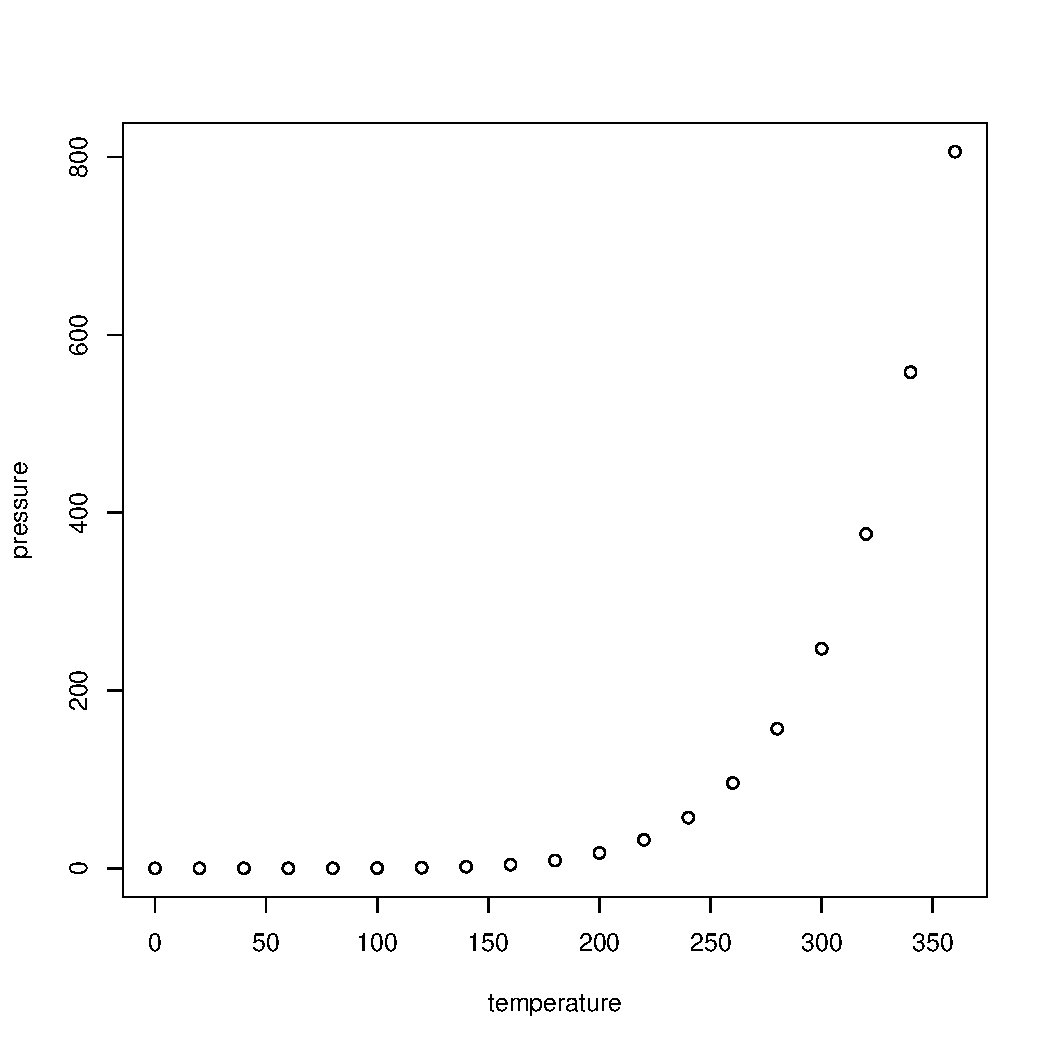
\includegraphics[width=\maxwidth]{figure/fig:pressure-1} 

\end{knitrout}
\caption{Figure Caption...we should turn "echo=False" in the R chunk options, but I left it true for now. (source: ??)} % define the caption, then the label.
\label{fig:pressure}

\end{figure}

\subsection{Imported Figures}

All figures and images that are imported should be put into the "images" sudirectory to keep stuff organized. Even better to create a subdirectory with your images, but we can naviagate as we go.

Figure \ref{fig:vadose} is a good example of this.

\begin{figure}
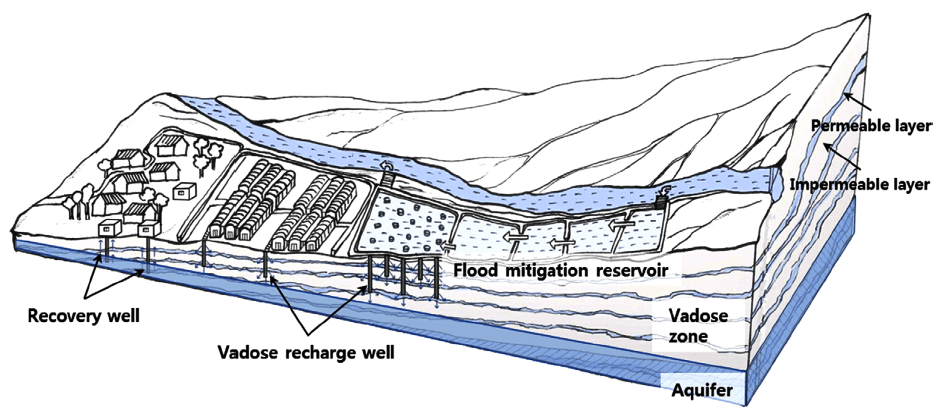
\includegraphics[width=\linewidth]{images/Lee_Vadose}
\caption{Vadose zone is neato}
\label{fig:vadose}
\end{figure}

In this case, I had to specify the width so it would fit on the page!  See the Rnw file for the code. Notice, I was also abel to "reference" the figure in the text.
\end{document}
